\chapter{Introduction}
\label{ch:intro}

Ce travail de Bachelor a pour but de réaliser un système de gestion de licences afin de garantir leur utilisation de manière licite.
En effet, dans le cadre de l'\textit{HEIG-VD}, certains logiciels sont fournis de manière gratuite mais sont soumis à certaines conditions d'utilisation.
Il faut noter notamment que leur utilisation à des fins personnelles ou commerciales est strictement interdite.
Actuellement, après avoir installé une application, il est impossible pour l'école de vérifier et encore moins de garantir que l'utilisation de ces logiciels est faite de manière licite.
L'idée de ce projet est donc de fournir à tous les étudiants de l'école une plateforme qui permet de lancer les applications sélectionnées de manière isolée et sécurisée.
Au départ, deux aspects principaux devaient ressortir de ce travail : une plateforme de gestion de licences et une distribution Linux optimisée pour lancer cette plateforme.
La suite d'actions permettant d'installer et d'utiliser cette distribution se fait comme suit :
\begin{itemize}
    \item L'installateur affiche un message d'avertissement pour faire une sauvegarde du disque courant.
    \item L'installation se déroule de la même manière que celle d'Ubuntu normal.
    \item Après le premier démarrage, la distribution demande les identifiants de l'utilisateur.
    \item Ces identifiants servent à configurer les différents services de l'école, comme la connexion au réseau, le VPN, les imprimantes, etc.
    \item Le système demande tous les six mois de rentrer les nouveaux identifiants afin de les mettre à jour. Il est aussi possible de le faire manuellement.
\end{itemize}

Pour le système de gestion de licences, une interface Web va être mise en place permettant d'assigner une liste d'applications disponible pour un étudiant.
En utilisant la technologie \acrshort{vnc}, il est possible de diffuser une application sur la plateforme depuis un serveur distant.
Chaque étudiant se voit donner un espace disque sur le serveur, à l'instar de \textit{eistore}, et peut interagir de manière contrôlée.
Le déroulement de cette connexion se ferait comme ceci :
\begin{figure}
    \centering
    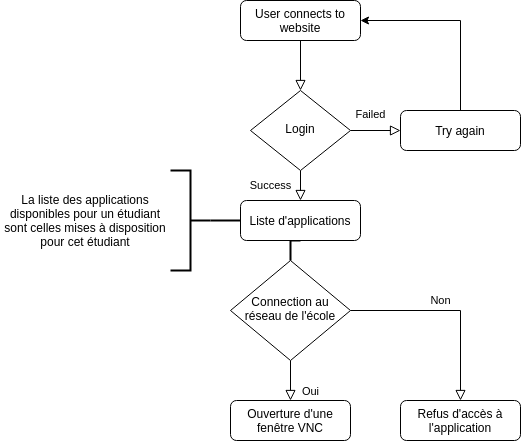
\includegraphics[scale=0.5]{images/VNC_use_case.png}
    \caption{Connexion au serveur}
    \label{fig:global_arch}
\end{figure}

\section{Plan du document}
Dans la suite de ce document, va être d'abord décrit les différentes recherches effectuées, les technologies appliquées et l'architecture de la distribution. 
Ensuite, nous allons aborder l'implémentation et les tests effectués sur la distribution.
La partie gestions de licences va être décrite avec les recherches et les décisions prises initialement.
Suite à une discussion avec un intervenant externe, il a été choisi qu'une direction autre que celle prise de base devra être suivie.
La phase de recherche et les décisions prises quant à cette direction sera explicitée.
Enfin, l'architecture, l'implémentation et les tests seront expliqués.
Finalement, une partie sera dédiée à l'analyse des résultats obtenus et une sur les travaux à réaliser et le futur de ce projet.


